\documentclass[tikz,border=8pt]{standalone}
\usepackage{amsmath}
\usepackage{pgfplots}
\pgfplotsset{compat=1.18}
\definecolor{ink}{HTML}{21352F}
\definecolor{teal}{HTML}{087F7B}
\definecolor{blue}{HTML}{4B77A8}
\definecolor{gold}{HTML}{C58B2A}
\definecolor{rose}{HTML}{B65A62}
\begin{document}
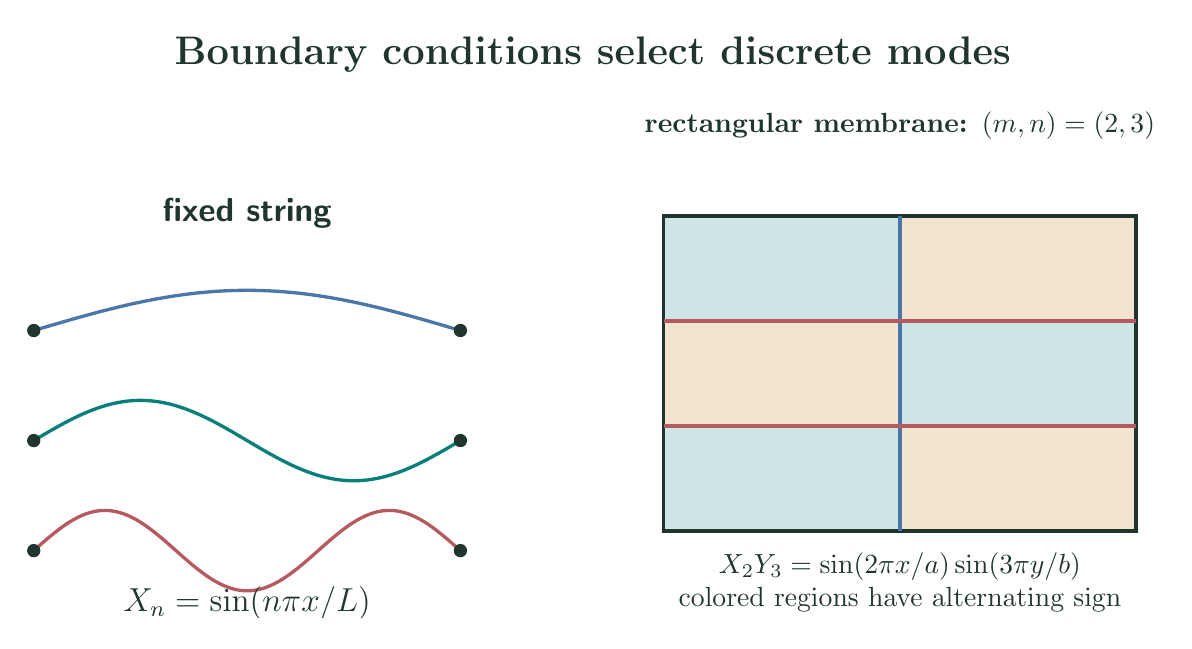
\begin{tikzpicture}[font=\large\sffamily,text=ink]
  \node[font=\bfseries\Large] at (0,4.15)
    {Boundary conditions select discrete modes};

  \begin{axis}[
    at={(-7.1cm,-3.0cm)},anchor=south west,
    width=7.0cm,height=6.2cm,
    axis lines=none,xmin=0,xmax=1,ymin=-.7,ymax=3.1,
    samples=150,domain=0:1,
    title={\bfseries fixed string}
  ]
    \addplot[blue,very thick] {0.42*sin(deg(pi*x))+2.3};
    \addplot[teal,very thick] {0.42*sin(deg(2*pi*x))+1.15};
    \addplot[rose,very thick] {0.42*sin(deg(3*pi*x))};
    \addplot[only marks,mark=*,mark size=2.2pt,ink]
      coordinates {(0,2.3)(1,2.3)(0,1.15)(1,1.15)(0,0)(1,0)};
    \node[anchor=east] at (axis cs:-.02,2.3) {$n=1$};
    \node[anchor=east] at (axis cs:-.02,1.15) {$n=2$};
    \node[anchor=east] at (axis cs:-.02,0) {$n=3$};
    \node at (axis cs:.5,-.55) {$X_n=\sin(n\pi x/L)$};
  \end{axis}

  \begin{scope}[xshift=3.9cm,yshift=.1cm]
    \node[font=\bfseries] at (0,3.15) {rectangular membrane: $(m,n)=(2,3)$};
    \foreach \i in {0,1}{
      \foreach \j in {0,1,2}{
        \pgfmathtruncatemacro{\parity}{mod(\i+\j,2)}
        \ifnum\parity=0
          \fill[teal!20] ({-3+3*\i},{-2+4*\j/3})
            rectangle ({-3+3*(\i+1)},{-2+4*(\j+1)/3});
        \else
          \fill[gold!22] ({-3+3*\i},{-2+4*\j/3})
            rectangle ({-3+3*(\i+1)},{-2+4*(\j+1)/3});
        \fi
      }
    }
    \draw[ink,very thick] (-3,-2) rectangle (3,2);
    \draw[blue,very thick] (0,-2)--(0,2);
    \draw[rose,very thick] (-3,-2/3)--(3,-2/3);
    \draw[rose,very thick] (-3,2/3)--(3,2/3);
    \node[font=\normalsize,align=center] at (0,-2.65)
      {$X_2Y_3=\sin(2\pi x/a)\sin(3\pi y/b)$\\
       colored regions have alternating sign};
  \end{scope}
\end{tikzpicture}
\end{document}
